\documentclass[UTF8]{ctexart}

\usepackage{graphicx}
\usepackage{amsmath}
\usepackage{xeCJK}
\usepackage{graphicx} %插入图片的宏包
\usepackage{float} %设置图片浮动位置的宏包
\usepackage{subfigure} %插入多图时用子图显示的宏包
\usepackage{geometry}
\usepackage[colorlinks,linkcolor=blue]{hyperref}


\geometry{a4paper,scale=0.8}
\CTEXsetup[format={\Large\bfseries}]{section}

\title{\textbf{用树状数组和快速排序算法求逆序对}}

\author{\CJKfamily{kai} 黄文\hbox{\scalebox{0.6}[1]{羽}\kern-.1em\scalebox{0.5}[1]{中}}\\3200100006}

\begin{document}

\maketitle

\section{问题描述}

 逆序对问题是指:给定一个不包含重复元素的数组$a$,问有多少对下标$(i,j)$,满足$i<j$,但是$a_i>a_j$

 自古以来,求逆序对就有一种经典的做法:利用归并排序的过程分治求解。然而,由于在C++下,排序可以调用STL库sort实现,且树状数组代码量很小,因此使用树状数组+排序也是一种广为流行的做法。

 尽管Linux Shell中没有自带的排序函数,但出于娱乐精神,本文作者仍然将使用Linux Shell脚本实现树状数组与快速排序,并用之求解逆序对问题。

\section{算法描述}

\subsection{树状数组}

树状数组是一种能支持$O(\log n)$时间内进行单点修改、区间求和的数据结构。下图展示了树状数组的工作原理。

\begin{figure}[H]
    \centering
    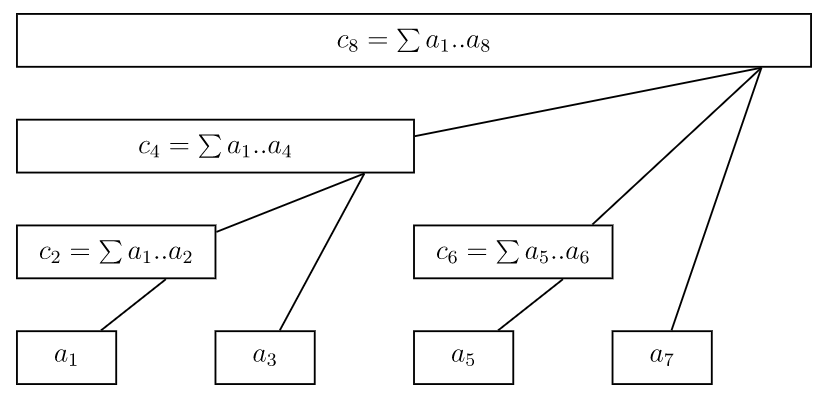
\includegraphics[width=0.5\textwidth]{img/bitarray.png}
    \caption{树状数组的工作原理(图源:OI Wiki)}
\end{figure}

在讨论实现之前,我们定义函数:$lowbit(x)=x\&-x$,这个函数返回$x$取值为1的最低二进制位对应的值。例如$10=(1010)_2$,则$lowbit(10)=2$。lowbit函数的shell脚本实现如下:

\begin{verbatim}
    # lowbit函数,返回最低二进制位
    lowbit(){
        lowbitret=$(($1&-$1))
    }
\end{verbatim}

观察上图不难发现,$a_x$的上级是$a_{x+lowbit(x)}$,当我们要令数组的$x$位置加$v$时,我们要将$a_x$的所有上级都加上$v$。实现该功能的函数shell脚本如下:
 
\begin{verbatim}
    # 使用 add p x 为数组p号位置的值增加x
    add(){
        pos=$1
        val=$2
        while [ $pos -le $n ]
        do
            bitarr[$pos]=$((${bitarr[$pos]}+$val))
            lowbit $pos
            pos=$(($pos+$lowbitret))
        done
    }
\end{verbatim}

对应地,当我们要查询数组$1,...,x$位置所有值之和时,我们从下标$x$出发,每次减去下标的$lowbit$值,经过的所有树状数组节点便能恰好覆盖$1,...,x$中的所有下标。其函数的Shell脚本实现如下:

\begin{verbatim}
    # 使用 qsum p x 查询[1,...,p]中所有数之和
    qsum(){
        pos=$1
        res=0
        while [ $pos -gt 0 ]
        do
            res=$(($res+${bitarr[$pos]}))
            lowbit $pos
            pos=$(($pos-$lowbitret))
        done
        qsumret=$res
    }
\end{verbatim}

以上就是树状数组原理的简单介绍及Shell脚本实现。关于原理的详细介绍请参考:\href{https://oi-wiki.org/ds/fenwick/}{树状数组 - OI Wiki}

\subsection{快速排序}

快速排序是一种平均$O(n\log n)$的不稳定排序方法,通过随机化可以避免最坏情况的出现,从而保证平均复杂度。以从大到小排序为例,其基本思想是:对于排序区间$[l,r]$,选择其中一个数$a_x$放在中间,将大于等于$a_x$的数都放在左侧,小于$a_x$的数都放在右侧。设最后$a_x$的位置为$k$,则对$[l,k-1]$和$[k+1,r]$区间进行递归的快排操作。

以下是用Shell脚本实现的带随机化的递归式快排函数。注意下面代码中还额外出现了$idx$数组,这是求逆序对所必要的,$idx[i]$表示排序后下标$i$的元素在原数组中的下标。在排序时,$idx$数组的交换要与$arr$数组的交换同步。

\begin{verbatim}
    # 快速排序,同时记录排序后元素的原位置
    qsort(){
        if [ $1 -lt $2 ]; then
            i=$1
            j=$2
            
            # 随机交换
            tmpid=$(($RANDOM%(j-i+1)+$i))
            tmpx=${arr[$i]}
            tmpy=${idx[$i]}
            arr[$i]=${arr[$tmpid]}
            idx[$i]=${idx[$tmpid]}
            arr[$tmpid]=$tmpx
            idx[$tmpid]=$tmpy
            
            k=${arr[$i]}
            tmpidx=${idx[$i]}
            while [ $i -lt $j ]; do
                while [ $i -lt $j ] && [ ${arr[$j]} -le $k ]; do
                    j=$(($j-1))
                done
                if [ $i -lt $j ]; then
                    idx[$i]=${idx[$j]}
                    arr[$i]=${arr[$j]}
                    i=$(($i+1))
                fi
                while [ $i -lt $j ] && [ ${arr[$i]} -gt $k ]; do
                    i=$(($i+1))
                done
                if [ $i -lt $j ]; then
                    idx[$j]=${idx[$i]}
                    arr[$j]=${arr[$i]}
                    j=$(($j-1))
                fi
            done
            arr[$i]=$k
            idx[$i]=$tmpidx
            qsort $1 $(($i-1))
            qsort $(($i+1)) $2
        fi
    }
\end{verbatim}

\subsection{主函数}

这一小节将介绍利用快速排序与树状数组求逆序对的算法与实现。

首先对输入的数组进行从大到小排序,同时用数组$idx[i]$记录排序后下标$i$的位置对应原数组的位置。然后按排序后的顺序遍历。

我们建立一个统计数组$c$,由于$idx[1,...,i-1]$都是值大于第$i$大的数对应的原位置,因此$idx[1],...,idx[i-1]$中小于$idx[i]$的数的个数就是以$idx[i]$为后者的逆序对数量。将$c$的$idx[1],...,idx[i-1]$位置都加上1,然后统计$c$下标$1,...,idx[i]$的所有元素之和即可。

这可以用树状数组实现,每次循环使用对$idx[i]$位置加1,然后利用qsum询问$1,...,idx[i]-1$中所有数之和。

主函数的Shell脚本实现如下:

\begin{verbatim}
    # 数组的总长
    read -p "请输入数组的长度:" n
    echo "请输入数组各元素(一行一个)"
    
    # 初始化各数组
    for ((i=1;i<=$n;i++)); do
        bitarr[$i]=0
        idx[$i]=$i
        read arr[$i]
    done
    
    # 排序后利用树状数组求逆序对数
    qsort 1 $n
    ans=0
    for ((i=1;i<=$n;i++)); do
        add ${idx[$i]} 1
        qsum $((${idx[$i]}-1))
        ans=$(($ans+$qsumret))
    done
    
    # 输出逆序对数和排序后的数组
    echo "逆序对数:" $ans
    echo "从大到小排序后数组:"
    for ((i=1;i<=$n;i++)); do
        echo ${arr[$i]}
    done
\end{verbatim}

\section{测试方法与测试结果}

\subsection{测试方法}

使用命令:

\begin{verbatim}
    bash good.sh
\end{verbatim}

运行程序。根据提示先输入数组长度,然后输入数组各元素(一行一个整数)。

也可以使用命令:

\begin{verbatim}
    bash good.sh < input > output
\end{verbatim}

进行文件输入输出。本文作者提供了一个1000个随机数的测试数据,在文件input中,直接执行上述命令即可测试这组数据。

\subsection{测试结果}

进行简单的测试,如下:

\begin{verbatim}
    wenchong@wenchong-ThinkPad-S2-3rd-Gen:~/桌面/code/MathSoftware/Homework-2$ bash good.sh
    请输入数组的长度:5
    请输入数组各元素(一行一个)
    1
    4
    5
    2
    3
    逆序对数: 4
    从大到小排序后数组:
    5
    4
    3
    2
    1
\end{verbatim}

测试结果正确。

进行文件输入输出测试,以input中的数据为例,结果请查看output文件。经检验,测试结果正确。

\section{细节说明}

\subsection{关于程序效率}

事实上,本程序采用的算法均为$O(n\log n)$的算法,理论速度应该非常快。然而,仅1000的数据量,却需要等肉眼可见的时间才能得出结果。经测试,这是因为shell的读写速度非常慢,大部分时间都花在了输入输出,因此算法的效率难以体现,更难以测试$10^5$级别的数据。这是一个遗憾。

\subsection{关于函数的返回值}

本程序中,qsum函数与lowbit函数其实都具有返回值,但没有显式地写出return语句。这是因为在调试过程中发现,return语句的返回值只能在$[0,255]$之间,超过这个区间将会返回0值。因此程序中定义了两个全局变量,以全局变量为媒介将函数需要返回的值传递出去。

\section{总结}

本程序的所有代码都在good.sh中,可以直接查看,并通过文章介绍的方法进行测试。

树状数组与快速排序并不是非常简单的任务,因此事实上并不适合使用shell脚本来实现,按照本文作者的经验,使用c语言或c++语言才是最为合适的方案,在程序执行效率和读写效率方面都更加地具有优势。

总之,本文使用shell脚本实现树状数组与快速排序,并用它们实现逆序对求解的程序,完全处于文章作者娱乐和炫技的需求,并不具有实际用途。希望读者在阅读本文时能感受到文章作者的娱乐精神,并通过阅读本文的代码感受到无上的快乐。

\end{document}